\chapter{Introduzione}

%%%%%%%%%%%%
% Content
%%%%%%%%%%%%
\section{Il mercato dell'energia}
La gestione centralizzata della rete elettrica è stata a lungo la scelta più ragionevole, ma adesso ha senso rivedere questo paradigma.
In passato, i grandi operatori elettrici erano anche quelli che producevano anche la quasi totalità dell'energia, gli unici ad avere a disposizione i mezzi per realizzare impianti costosi e complessi.
Ad effettuarne poi la distribuzione sono poi i \gls{tso}, spesso con coperture nazionali, come la italiana Terna \cite{art:terna-role}. \\
La situazione odierna, tuttavia, è diversa.
Negli anni abbiamo assistito ad una riduzione progressiva del costo degli impianti per la produzione di energia rinnovabile, 
anche grazie a regolamentazioni estremamente favorevoli \cite{art:renewable-energy-regulations}. \\
La conseguenza è una diffusione sempre più capillare di piccoli produttori di energia elettrica, 
che attraverso piccoli impianti, spesso domestici, sono in grado di offrire un contributo attivo alla rete \cite{art:renewable-energy-increment}. \\
Ad essi si aggiungono dispositivi come veicoli elettrici e nuovi sistemi di stoccaggio di energia, i quali, se ben gestiti, 
possono offrire un servizio utile all'intera rete elettrica. \\
Tutti questi dispositivi, definiti \gls{der}, introducono la necessità di un flusso bidirezionale di energia che li includa come agenti attivi \cite{art:enel-der}. \\
Inoltre, la natura variabile e difficile da prevedere della maggior parte delle fonti di energia rinnovabile o \gls{res} ne richiede una gestione flessibile, 
in grado di garantire robustezza e stabilità all'intera rete \cite{art:blockchain-der}. \\

La gestione di queste piccole realtà, mal si sposa con l'attuale struttura centralizzata, e impone un cambio di paradigma verso un'architettura distribuita, 
in grado di includere i \gls{der} e mettere a più stretto contatto produttore e consumatore.

\begin{figure}[h]
    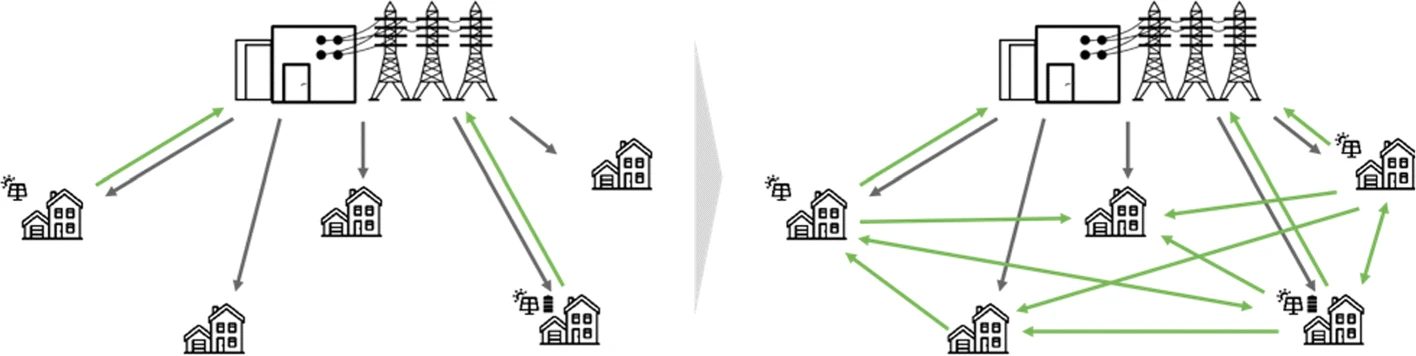
\includegraphics[width=9cm]{p2pgrid}
    \centering
    \caption{Da rete da centralizzata a rete distribuita \cite{img:p2pgrid}}
    \label{lab:p2pgrid}
\end{figure}


\section{La tecnologia delle blockchain}
La tecnologia delle blockchain esiste già da parecchi anni, ma negli ultimi tempi ha ricevuto crescenti attenzioni da studiosi e industrie, intenzionate a sfruttarne a pieno il potenziale. \\
Tralasciando i dettagli più tecnici della tecnologia, che è possibile approfondire in pubblicazioni come quelle referenziate in \cite{art:blockchain} e \cite{art:blockchain-for-industry}, 
la blockchain può essere vista come una lista di transazioni pubblica, decentralizzata e immutabile, se non per l'aggiunta di nuove transazioni, della quale chiunque può possedere una copia. \\
L'integrità e la correttezza delle transazioni vengono garantite dagli algoritmi crittografici, che rendono molto facile verificare la validità della transazione. \\
Ciò permette l'interazione di una qualsiasi entità con le altre senza che questa debba fare affidamento su nient'altro che l'algoritmo di consenso distribuito che governa la blockchain, eliminando la necessità di un intermediario fra le parti. 
Il risultato è una rete distribuita \gls{p2p} estremamente robusta che si presta a molteplici applicazioni. \\
A rendere ancora più appetibile questa tecnologia sono gli smart contracts, presenti in reti come Ethereum \cite{wiki:eth-smart-contracts}. Semplificando, si tratta di veri e propri software rilasciati sulla blockchain 
in grado di compiere svariate azioni in maniera automatica seguendo la loro programmazione.